\documentclass{article}
\usepackage[english]{babel}
\usepackage[a4paper,top=2.54cm,bottom=2.54cm,left=2.54cm,right=2.54cm,marginparwidth=1.75cm]{geometry}
\usepackage{amsmath}
\usepackage{graphicx}
\usepackage{amsfonts}
\usepackage{amssymb}
\usepackage{enumerate}
\usepackage{enumitem}
\usepackage[colorlinks=true, allcolors=blue]{hyperref}
\title{Linear Algebra: Homework 9}
\begin{document}
\maketitle
\subsection*{Question 1.}
Determine which pair of vectors are orthogonal:
\begin{enumerate}[label=(\arabic*)]
    \item $\mathbf{u}=\left[\begin{array}{r}12\\3\\-5\end{array}\right]$, $\mathbf{v}=\left[\begin{array}{r}2\\-3\\3\end{array}\right]$; \item $\mathbf{u}=\left[\begin{array}{r}-3\\7\\4\\0\end{array}\right]$, $\mathbf{v}=\left[\begin{array}{r}1\\-8\\15\\-7\end{array}\right]$.
\end{enumerate}
\subsection*{Solution 1.}
\begin{enumerate} [label=(\arabic*)]
    \item \[\langle \mathbf{u},\mathbf{v}\rangle =12\times 2+3\times (-3)+(-5)\times 3=24-9-15=0\]
    Hence $\mathbf{u}\perp \mathbf{v}$.
    \item \[\langle \mathbf{u},\mathbf{v}\rangle =(-3)\times 1+7\times (-8)+4\times 15+0\times(-7)=-3-56+60+0=1\]
    Hence $\mathbf{u}$ $\not\perp$  $\mathbf{v}$ .
\end{enumerate}
\subsection*{Question 2.}
Mark each statement true or false, and justify your answer.
\begin{enumerate} [label=(\arabic*)]
    \item $\langle \mathbf{v},\mathbf{v}\rangle=||\mathbf{v}||^2$.
    \item For any scalar $c$, $\langle \mathbf{u},c\mathbf{v}\rangle=c\langle \mathbf{u},\mathbf{v}\rangle$.
    \item If the distance from $\mathbf{u}$ to $\mathbf{v}$ equals the distance from $\mathbf{u}$ to $\mathbf{-v}$, then $\mathbf{u}$ and $\mathbf{v}$ are orthogonal.
    \item For a square matrix $A$, vectors in Col($A$) are orthogonal to vectors in Nul$(A)$.
    \item If vectors $\mathbf{v}_1,\cdots,\mathbf{v}_p$ span a subspace $W$, and if $\mathbf{x}$ is orthogonal to each $\mathbf{v}_i$ for $i=1,\cdots,p$, then $\mathbf{x}$ is in $W^\perp$.
\end{enumerate}
\subsection*{Solution 2.}
The following assumes $\mathbf{u},\mathbf{v}\in\mathbf{R}^n$.
\begin{enumerate} [label=(\arabic*)]
    \item True.
    \[\langle \mathbf{v},\mathbf{v}\rangle=\mathbf{v}^T\mathbf{v}=\sum_{i=1}^n v_i^2=||\mathbf{v}||^2\text{      }\blacksquare\]
    \item True.
    \[\langle\mathbf{u},c\mathbf{v}\rangle=\mathbf{u}^T(c\mathbf{v})=c\mathbf{u}^T\mathbf{v}=c\langle\mathbf{u},\mathbf{v}\rangle \text{      }\blacksquare\]
    \item True. The statement can be rewritten as
    \[||\mathbf{u}-\mathbf{v}||=||\mathbf{u}-(-\mathbf{v})||
    \Leftrightarrow ||\mathbf{u}-\mathbf{v}||^2=||\mathbf{u}+\mathbf{v}||^2\]
    By distributive property of inner product over vector addition,
    \[||\mathbf{u}-\mathbf{v}||^2-||\mathbf{u}+\mathbf{v}||^2
    =\langle \mathbf{u}-\mathbf{v},\mathbf{u}-\mathbf{v}\rangle-\langle \mathbf{u}+\mathbf{v},\mathbf{u}+\mathbf{v}\rangle
    \]
    \[=\langle \mathbf{u},\mathbf{u}\rangle-\langle\mathbf{u}-\mathbf{v}\rangle-\langle \mathbf{v},\mathbf{u}\rangle+\langle\mathbf{v},\mathbf{v}\rangle-\langle \mathbf{u},\mathbf{u}\rangle-\langle\mathbf{u}-\mathbf{v}\rangle-\langle \mathbf{v},\mathbf{u}\rangle-\langle\mathbf{v},\mathbf{v}\rangle\]
    \[=-2\langle \mathbf{u},\mathbf{v}\rangle-2\langle \mathbf{v},\mathbf{u}\rangle
    =-4\langle \mathbf{u},\mathbf{v}\rangle=0
    \]
    \[\Leftrightarrow \langle \mathbf{u},\mathbf{v}\rangle=0\text{      }\blacksquare\]
    \item False.
    In fact, Col($A^T$)=Nul($A)^\perp$
    Let $A=\left[\begin{array}{rr}
    0 & 1 \\
    0 & 0
    \end{array}\right]$. Then $\left[\begin{array}{r} 1 \\ 0 \end{array}\right]\in$ Nul($A$).
    However, referring to the second column of $A$,
    \[\left[\begin{array}{rr} 1 &0\end{array}\right]\left[\begin{array}{r} 1 \\ 0 \end{array}\right]=1\neq 0,\]
    which disproved the statement.
    \item True. $W^\perp$ is defined as
\[W^\perp =\{\mathbf{v}\in\mathbf{R}^n:(\forall \mathbf{w}\in W) \langle \mathbf{v},\mathbf{w}\rangle=0\}\]
    \[W^\perp =\{\mathbf{x}\in\mathbf{R}^n: \langle \mathbf{x},\sum_{i=1}^p c_i\mathbf{v}_i\rangle=0,c_i\in\mathbf{R}\}\]
    \[=\{\mathbf{x}\in\mathbf{R}^n: \sum_{i=1}^p c_i\langle \mathbf{x},\mathbf{v}_i\rangle=0,c_i\in\mathbf{R}\}\]
    Hence $\forall\mathbf{x}\in\mathbf{R}^n$ such that $\langle\mathbf{x},\mathbf{v}_i\rangle=0$ for $i\in\{1,2,\cdots,p\}$, 
    \[\sum_{i=1}^p c_i\langle \mathbf{x},\mathbf{v}_i\rangle=0\Rightarrow \mathbf{x}\in W^\perp\]
\end{enumerate}
\subsection*{Question 3.}
Verify the \textit{parallelogram law} for vectors $\mathbf{u}$ and $\mathbf{v}$ in $\mathbf{R}^n$.
\[||\mathbf{u}+\mathbf{v}||^2+||\mathbf{u}-\mathbf{v}||^2=2(||\mathbf{u}||^2+||\mathbf{v}||^2).\]
\subsection*{Solution 3.}
By distributive property of inner product over vector addition,
    \[||\mathbf{u}+\mathbf{v}||^2+||\mathbf{u}-\mathbf{v}||^2=\langle \mathbf{u}+\mathbf{v},\mathbf{u}+\mathbf{v}\rangle+\langle \mathbf{u}-\mathbf{v},\mathbf{u}-\mathbf{v}\rangle
    \]
    \[=\langle \mathbf{u},\mathbf{u}\rangle+\langle\mathbf{u},\mathbf{v}\rangle+\langle \mathbf{v},\mathbf{u}\rangle+\langle\mathbf{v},\mathbf{v}\rangle+\langle \mathbf{u},\mathbf{u}\rangle-\langle\mathbf{u}-\mathbf{v}\rangle-\langle \mathbf{v},\mathbf{u}\rangle+\langle\mathbf{v},\mathbf{v}\rangle\]
    \[=2\langle \mathbf{u},\mathbf{u}\rangle+2\langle \mathbf{v},\mathbf{v}\rangle
    =2(||\mathbf{u}||^2+||\mathbf{v}||^2)\text{     } \blacksquare
    \]
\subsection*{Question 4.}
Show that if $\mathbf{x}$ is in both $W$ and $W^\perp$, then $\mathbf{x}=0$.
\subsection*{Solution 4.}
Let $W\subset \mathbf{R}^n$.\newline
$W^\perp$ is defined as
\[W^\perp =\{\mathbf{v}\in\mathbf{R}^n:(\forall \mathbf{w}\in W) \langle \mathbf{v},\mathbf{w}\rangle=0\}\]
Hence, \[\forall \mathbf{x}\in (W\cap W^\perp),\langle \mathbf{x},\mathbf{x}\rangle=0\Rightarrow \mathbf{x}=0\]

\subsection*{Question 5.}
Determine which set of vectors are orthogonal:
\begin{enumerate}[label=(\arabic*)]
    \item $\left[\begin{array}{r}2\\-7\\-1\end{array}\right]$, $\left[\begin{array}{r}-6\\-3\\9\end{array}\right]$,$\left[\begin{array}{r}3\\1\\-1\end{array}\right]$.
    \item $\left[\begin{array}{r}3\\-2\\1\\3\end{array}\right]$, $\left[\begin{array}{r}-1\\3\\-3\\4\end{array}\right]$,$\left[\begin{array}{r}3\\8\\7\\0\end{array}\right]$.
\end{enumerate}
\subsection*{Solution 5.}
\begin{enumerate}[label=(\arabic*)]
    \item 
    \[\left[\begin{array}{rrr}-6&-3&9\end{array}\right]\left[\begin{array}{r}3\\1\\-1\end{array}\right]=-18-3-9=-30\neq 0\]
    Hence this set of vectors is not orthogonal.
    \item
    \[\left[\begin{array}{rrrr}3&-2&1&3\end{array}\right]\left[\begin{array}{r}-1\\3\\-3\\4\end{array}\right]=-3-6-3+12=0,\]
    \[\left[\begin{array}{rrrr}3&-2&1&3\end{array}\right]\left[\begin{array}{r}3\\8\\7\\0\end{array}\right]=9-16+7+0=0,\]
    \[\left[\begin{array}{rrrr}-1&3&-3&4\end{array}\right]\left[\begin{array}{r}3\\8\\7\\0\end{array}\right]=-3+24-21+0=0\]
    Hence this set of vectors is orthogonal.
\end{enumerate}
\subsection*{Question 6.}
Show that \{$\mathbf{u}_1,\mathbf{u}_2,\mathbf{u}_3$\} is an orthogonal basis for $\mathbf{R}^2$ or $\mathbf{R}^3$ respectively. Then express $\mathbf{x}$ as a linear combination of the $\mathbf{u}_i$'s.
\begin{enumerate}[label=(\arabic*)]
    \item $\mathbf{u}_1=\left[\begin{array}{r}2\\-3\end{array}\right]$, $\mathbf{u}_2=\left[\begin{array}{r}6\\4\end{array}\right]$, and $\mathbf{x}=\left[\begin{array}{r}9\\-7\end{array}\right]$.
    \item $\mathbf{u}_1=\left[\begin{array}{r}1\\0\\1\end{array}\right]$, $\mathbf{u}_2=\left[\begin{array}{r}-1\\4\\1\end{array}\right]$, $\mathbf{u}_3=\left[\begin{array}{r}2\\1\\-2\end{array}\right]$, and $\mathbf{x}=\left[\begin{array}{r}8\\-4\\-3\end{array}\right]$.
    
\end{enumerate}
\subsection*{Solution 6.}
\begin{enumerate}[label=(\arabic*)]
    \item Orthogonality:\[\langle \mathbf{u}_1,\mathbf{u}_2\rangle=12-12=0\]
    Let $\mathbf{x}=a\mathbf{u}_1+b\mathbf{u}_2$, then
    \[\left[\begin{array}{r}a\\b\end{array}\right]=\left[\begin{array}{rr}2&6\\-3&4\end{array}\right]^{-1}\left[\begin{array}{r}9\\-7\end{array}\right]=\frac{1}{26}\left[\begin{array}{rr}4&-6\\3&2\end{array}\right]\left[\begin{array}{r}9\\-7\end{array}\right]=\left[\begin{array}{r}3\\1/2\end{array}\right],\]
    So
    \[\mathbf{x}=3\mathbf{u}_1+\frac{1}{2}\mathbf{u}_2\]
    \item Orthognality:
    \[\langle \mathbf{u}_1,\mathbf{u}_2\rangle=-1+1=0\]
    \[\langle \mathbf{u}_1,\mathbf{u}_3\rangle=2-2=0\]
    \[\langle \mathbf{u}_2,\mathbf{u}_3\rangle=-2+4-2=0\]
    Let $\mathbf{x}=a\mathbf{u}_1+b\mathbf{u}_2+c\mathbf{u}_3$, then find $a,b,c$ by Gauss-Jordan:
    \[\left[\begin{array}{rrrr}
1 & -1 & 2 & 8 \\
0 &  4 & 1 & -4\\
1 & 1 & -2 & -3
    \end{array}\right]\sim\left[\begin{array}{rrrr}
1 & -1 & 2 & 8 \\
0 &  4 & 1 & -4\\
0 & 2 & -4 & -11
    \end{array}\right]\sim\left[\begin{array}{rrrr}
1 & -1 & 2 & 8 \\
0 &  4 & 1 & -4\\
0 & 0 & -9/2 & -9
    \end{array}\right],\]
    So $c=2,b=(-4-2)/4=-3/2,a=8-4-3/2=5/2$,
    \[\mathbf{x}=\frac{5}{2}\mathbf{u}_1-\frac{3}{2}\mathbf{u}_2+2\mathbf{u}_3\]
\end{enumerate}
\subsection*{Question 7.}
\begin{enumerate} [label=(\arabic*)]
    \item Let $\mathbf{y}=\left[\begin{array}{r}2\\3\end{array}\right]$ and $\mathbf{u}=\left[\begin{array}{r}4\\-7\end{array}\right]$. Write $\mathbf{y}$ as the sum of two orthogonal vectors, one in Span\{$\mathbf{u}$\} and the other orthogonal to $\mathbf{u}$.
    \item Let $\mathbf{y}=\left[\begin{array}{r}3\\1\end{array}\right]$ and $\mathbf{u}=\left[\begin{array}{r}8\\6\end{array}\right]$. Compute the distance from $\mathbf{y}$ to the line through $\mathbf{u}$ and the origin.
\end{enumerate}
\subsection*{Solution 7.}
\begin{enumerate} [label=(\arabic*)]
    \item Let $\mathbf{v}=\left[\begin{array}{r}7\\4\end{array}\right]$.
    \[\langle \mathbf{u},\mathbf{v}\rangle=28-28=0\Rightarrow \mathbf{u}\perp\mathbf{v}.\]
    Let $\mathbf{y}=a\mathbf{u}+b\mathbf{v}$, then 
    \[\left[\begin{array}{r}a\\b\end{array}\right]=\left[\begin{array}{rr}4&7\\-7&4\end{array}\right]^{-1}\left[\begin{array}{r}2\\3\end{array}\right]=\frac{1}{65}\left[\begin{array}{rr}4&-7\\7&4\end{array}\right]\left[\begin{array}{r}2\\3\end{array}\right]=\left[\begin{array}{r}-1/5\\2/5\end{array}\right],\]
    So
    \[\mathbf{y}=-\frac{1}{5} \mathbf{u}+\frac{2}{5}\mathbf{v},\text{ where }\mathbf{v}=\left[\begin{array}{r}7\\4\end{array}\right]\]
    \item Distance
    \[=||\mathbf{y}-\frac{\langle \mathbf{u},\mathbf{y}\rangle}{||\mathbf{u}||^2}\mathbf{u}||\]
    \[=\left\vert\left\vert\left[\begin{array}{r} 3\\1\end{array}\right]-\frac{30}{100}\mathbf{u}\right\vert\right\vert=\sqrt{(3-2.4)^2+(1-1.8)^2}=1\]
\end{enumerate}
\subsection*{Question 8.}
\begin{enumerate} [label=(\arabic*)]
    \item Let $U$ and $V$ be $n\times n$ orthogonal matrices. Explain why $UV$ remains an orthogonal matrix.
    \item Let $U$ be an orthogonal matrix, and construct $V$ by interchanging some of the columns of $U$. Explain why $V$ is an orthogonal matrix.
\end{enumerate}
\subsection*{Solution 8.}
Let $V\in\mathbf{R}^{n\times n}$. $V$ is an orthogonal matrix iff $V^TV=I_n$.
\begin{enumerate}[label=(\arabic*)]
    \item The proof follows by the fact that 
    \[(UV)^T(UV)=V^TU^T UV=V^T I_n V=V^TV=I_n\square\]
    \item Let $\pi:\{1,2,\cdots,n\}\to\{1,2,\cdots,n\}$
    represented by
    \[\left(\begin{array}{rrrr}
    1 & 2 & \cdots & n \\
    \pi(1) & \pi(2) & \cdots & \pi(n)
    \end{array}\right)\]
    be a permutation of the columns of $U$ that constructs $V$. Then,
    \[P=[\begin{array}{rrrr}\mathbf{e}_{\pi(1)}&\mathbf{e}_{\pi(2)}&\cdots&\mathbf{e}_{\pi(n)}\end{array}]\]
    $P$ is an orthogonal matrix, since the columns of $P$ are $\{\mathbf{e}_{\pi(1)},\mathbf{e}_{\pi(2)},\cdots,\mathbf{e}_{\pi(n)}\}$ is just the rearrangement of the standard basis, which is orthogonal.\newline
    Then we have $V=UP$. $U$ and $P$ are orthogonal matrices, by (1) $V$ is also an orthogonal matrix.  $\blacksquare$
\end{enumerate}
\subsection*{Question 9.}
Given $\mathbf{u}\neq 0$ in $\mathbf{R}^n$, let $L=$Span\{$\mathbf{u}$\}. For $\mathbf{y}\in\mathbf{R}^n$, let Refl$_L(\mathbf{y})$ be the reflection of $\mathbf{y}$ with respect to $L$ as shown in the figure.\newline
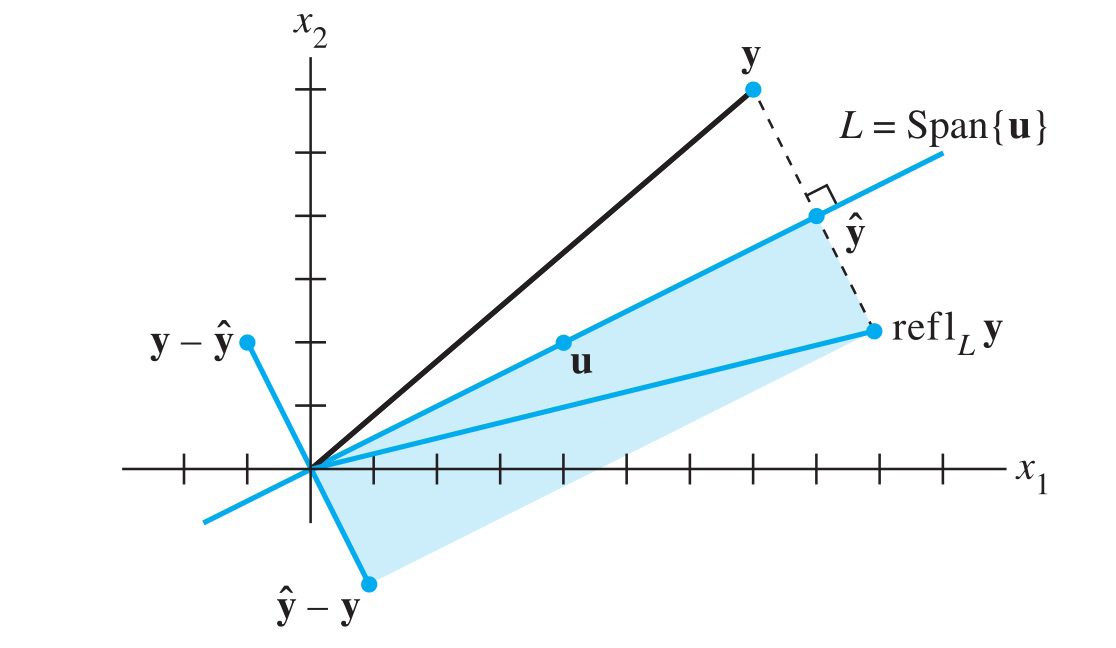
\includegraphics[scale=0.5]{img/20211206_linalg_HW9_Fig_1.PNG}\newline
Show that 
\[\text{Refl}_L(\mathbf{y})=2\cdot \text{proj}_L(\mathbf{y})-\mathbf{y},\]
and that $\mathbf{y}\mapsto$ Refl$_L(\mathbf{y})$ defines a linear transformation.
\subsection*{Solution 9.}
By definition, 
\[\text{proj}_L(\mathbf{y})=\mathbf{u}(\mathbf{u}^T\mathbf{u})^{-1}\mathbf{u}^T\mathbf{y},\]
So, if Refl$_{L}(\mathbf{y})$ represents the image of $y$ formed by reflection w.r.t. $L$,
\[\mathbf{y}-\text{proj}_L(\mathbf{y})=-(\text{Refl}_L(\mathbf{y})-\text{proj}_L(\mathbf{y}))\]
\[\Leftrightarrow \text{Refl}_L(\mathbf{y})=2\cdot \text{proj}_L(\mathbf{y})-\mathbf{y},\square\]
Linearity of reflection can be shown by 
\[\text{Refl}_L(a\mathbf{x}+b\mathbf{y})=2\mathbf{u}(\mathbf{u}^T\mathbf{u})^{-1}\mathbf{u}^T(a\mathbf{x}+b\mathbf{y})-(a\mathbf{x}+b\mathbf{y})\]
\[=a(2\mathbf{u}(\mathbf{u}^T\mathbf{u})^{-1}\mathbf{u}^T\mathbf{x}-\mathbf{x})+b(2\mathbf{u}(\mathbf{u}^T\mathbf{u})^{-1}\mathbf{u}^T\mathbf{y}-\mathbf{y})\]
\[=a\cdot \text{Refl}_L(\mathbf{x})+b\cdot \text{Refl}_L(\mathbf{y})\blacksquare\]
\end{document}